
\section{Energy-Optimal Configurations for Single-Node HPC Applications\\
%{\footnotesize \textsuperscript{*}Note: Sub-titles are not captured in Xplore and should not be used}
%\thanks{Identify applicable funding agency here. If none, delete this.}
}

% Energy efficiency is a growing concern for modern computing, especially for High-Performance Computing (HPC) due to operational costs and the environmental impact. We propose a methodology to find the best energy-efficient configurations to run single-node applications in an HPC environment using an application-agnostic power model of the architecture and an architecture-aware performance model of the application. The operating frequency and number of active cores are the configuration parameters. This method differs from frequency scaling algorithms that do not have any previous information on the performance behavior of the application or the power consumption profile of the architecture. We characterize the application performance using Support Vector Regression. The power consumption is estimated by modeling the dynamic and static power consumed by CMOS transistors using a computation-intensive program to stress the architecture. The estimated energy-optimal configuration is computed by minimizing the product of the power model and the performance model's outcomes. The results obtained using four PARSEC applications with five different inputs show that the proposed approach was able to find configurations that used about 14$\times$ less energy when compared to the worst case of the default Linux governor for voltage and frequency scaling. When compared to the best case of this governor, the proposed approach saved up to 23\% on energy consumption, with an overall average of 6\% less energy.
% 150 words abstract
Energy efficiency is a growing concern for modern computing, especially for HPC due to operational costs and the environmental impact, considering that processors have an important role in this energy consumption. In this work, we propose a methodology to find energy-optimal frequency and number of active cores to run single-node HPC applications using an application-agnostic power model of the architecture and an architecture-aware performance model of the application. We characterize the application performance using machine learning, specifically the "Support Vector Regression" algorithm. Besides that, the power consumption is estimated by modeling CMOS dynamic and static power without knowledge of the application. So, The energy-optimal configuration is estimated by minimizing the product these two models outcomes, the power model and the performance model. Then, the final model can be used to find better frequency and number of cores to aim energy efficiency application execution. Results were obtained for four PARSEC applications and, with five different inputs shows that the proposed approach used substantially less energy when compared to the DVFS governor, in best cases and worst cases.


\section{Introduction} \label{sec:introduction}
Processors are the main contributor to the power consumption of High-Performance Computing (HPC) servers. They contribute between 20 and 40\% to the total server’s power draw~\cite{Fan2007}. Google's servers showed that during peak utilization processors consumed about 42\% of the overall server’s power consumption~\cite{Barroso2007}. Reducing processor power consumption is an effective approach to reduce the whole system's power consumption.  Therefore, modern processors incorporate several features for power management such as independent processing cores that can be disabled by the operating system~\cite{Rotem2012}, clock gating techniques for reducing the dynamic power dissipation of synchronous circuits~\cite{Srinivasan2015} and Dynamic Voltage and Frequency Scaling (DVFS)~\cite{Mittal2014}.

DVFS has been demonstrated to be a very effective technique for reducing the power consumption of processors \cite{Hackenberg2015, Dzhagaryan2014, Hahnel2012, Basmadjian2012, Travers2015, Miyoshi2002, Anghel2011, Pietri2014}. The technique tries to optimize power consumption by adjusting the frequency according to the current load of the processor. Generally, the frequency scales with the intensity of the load and the voltage scales to the minimum value that enables the selected frequency. Among other aspects, DVFS helps in reducing energy consumption because it allows memory-bounded programs to be executed more efficiently \cite{Spiga2006}. Nonetheless, aspects such as load variability may compromise the effectiveness of DVFS. Another important aspect that is typically not taken into account is the number of processing cores to be used by a parallel program. This choice is left to the user, which often is not trivial as shown in this paper.% the power consumption but increasing the execution time. This way is not guaranteed that the energy consumption will be the lower since energy depends on the power and time, there might be a configuration with higher power consumption that can lead to less energy consumed because of the execution time is lower.

We propose a methodology to find the operating frequency and number of active cores that minimize the total energy used to execute an HPC application on a single shared-memory HPC node.

The methodology uses an application-agnostic power model and an architecture-specific application characterization to model performance. The power model is based on the modeling of Complementary Metal-Oxide-Semiconductor (CMOS) logic in the function of the operating frequency \cite{Sarwar1997}. It models both dynamic and static power. Besides operating frequency, the power model is also parametric to the number of active sockets and the number of active cores per socket. 

Performance is modeled by characterizing the application on the target architecture. The idea is to predict the performance of the application at any given configuration. The model takes as inputs the operating frequency, the number of active cores and the input size. The modeling is done using a supervised learning method for regression called Support Vector Regression (SVR)~\cite{Smola2004}.

To find the optimal-energy configurations, the algorithm minimizes the product of outcomes of the power and performance models. This approach was validated on four PARSEC applications~\cite{Bienia2008} and compared to the \emph{Ondemand} governor, which is the default DVFS scheme for the Linux operating system. The results show that the proposed approach was able to find configurations that used about 14$\times$ less energy when compared to the worst case of the Ondemand governor. When compared to the best case of this DVFS scheme, i.e. when the user guesses the optimal number of cores to be used, the proposed approach was able to find configurations that used as much as 18.7\% less energy to execute the target application. The overall average energy saving reached 5.7\% for the proposed approach when compared to the best case and 88.8\% when compared to the worst case.

% TODO: Terminar de detalhar quando fechar a versão final das seções

The rest of this paper is organized as follows. Section~\ref{sec:models} presents the proposed models for power, performance, and energy. The experimental setup and the fitting of the models are described in Section~\ref{sec:experimentalsetup}. In Section~\ref{sec:experimentsresults}, the results of applying the proposed approach to four PARSEC applications are presented. Related works are presented in Section~\ref{sec:relatedwork}. Finally, conclusions are drawn and future work is proposed in Section\ref{sec:conclusion}.

% \section{Theoretical background} \label{Theoretical_background}
% %In the following subsections we present a background on how the DVFS control works and describe how to monitor of power information in real time.

% \subsection{DVFS} \label{DVFS}
% The DVFS implementation complies with the Advanced Configuration and Power Interface (ACPI) \cite{Wikipedia2010} standard which is adopted by operating systems to configure hardware components related to power management. In this standard two states are defined, the C and P states, which are important to the processor frequency and voltage control.

% The C state optimizes the power consumption when the processor is not executing any instructions. This state has several levels. The processor initially starts at C0 level, where the Central Processing Unit (CPU) is fully activated. If the CPU is idle for a specified time, then it moves to the next level, C1, where some CPU functionalities are disabled. After spending some time on the C1 level, the processor passes to the next level where more functionalities are disabled, and so on. ACPI defines four levels, but, manufacturers can define additional ones.

% The P state optimizes the voltage and the frequency during the active execution. It starts at the P0 level, with the highest frequency and voltage possible.  At the P1 level, both the frequency and voltage are decreased, and this goes on until the last level is reached with the lowest possible values. The ACPI standard does not specify the number of the P levels, so this is a manufacturers' choice.

% The P and C states can be controlled by interfaces mediated by drivers available on the operating system. The Linux kernel has many drivers available developed by the CPU manufacturers and the community \cite{Brown2005}. The default driver is the "acpi-cpufreq'' that uses policies implemented by so-called governors that dynamically decide the frequency values. Some of the governors available are Performance, Powersave, Ondemand, Conservative and Userspace. Performance and Powersave are static, and they set the frequency to the maximum and minimum allowed values, respectively. Ondemand and Conservative implementing algorithms to estimate the CPU required capacity and adjust the processor frequency accordingly. Finally, Userspace allows the user to specify the frequency.

% \subsection{IPMI} \label{IPMI}

% The Intelligent Platform Management Interface(IPMI) is a set of interfaces used by HPC system administrators. These allow for out-of-band management of computer systems and platform-status monitoring through local network \cite{November2013}. It can monitor variables and resources such as the system's temperature, voltage, fans and power supplies, with independent sensors attach to the hardware.

% The system consists of the main controller, called the baseboard management controller (BMC), and other management controllers distributed among different system modules, as shown in figure \ref{fig:ipmi_diagram}.

% \begin{figure}[H]
% \centerline{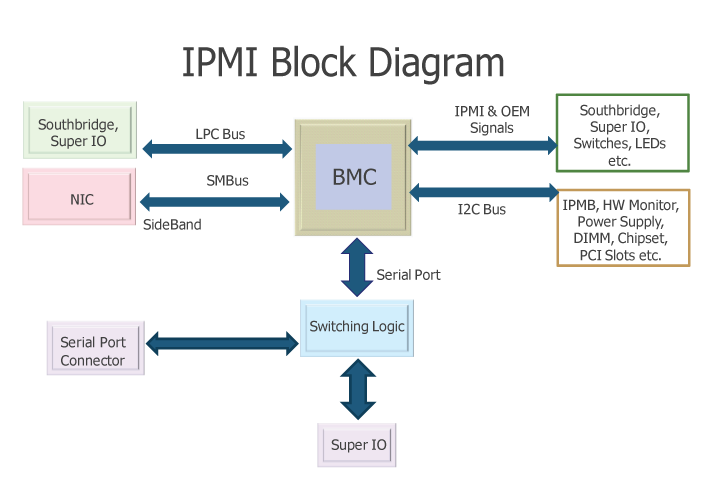
\includegraphics[width=\columnwidth]{figures/IPMI-Block-Diagram.png}}
% \caption{IPMI block diagram, this image was taken from http://pt.wikipedia.org }
% \label{fig:ipmi_diagram}
% \end{figure}

% %The BMC operate independent of the operating system and his access can be through HTTP protocol or using a tool provided by the manufacturer.

\section{Models} \label{sec:models}
In this Section, we present the proposed power and performance models that are used to estimate the minimum-energy consumption configuration.

\subsection{Power Model} \label{sec:powermodel}
Some of the main factors that contribute to the CPU power consumption are the dynamic power consumption, the short-circuit power consumption, and the power loss due to the current leakage of transistors, \cite{Rauber2014, Goel2016, Du2017, Gonzalez1997}. The complexity of the circuits of modern processors makes it very difficult to model their power consumption accurately. A viable approach for modeling the CPU's power draw is to model their building components, which are mainly made out of CMOS logic gates. Thus, modeling the power consumption for one logic gate and multiplying this by the total number of gates reduces the complexity of modeling the internal circuits but still provides the sufficient accuracy needed for making optimization decisions.

%The modern technology to construct logic gates is the CMOS, and t
There are three main components of power dissipation in digital CMOS circuits,
\begin{equation}
P_{total}=P_{static}+P_{leak}+P_{dynamic} \label{eq_totalPower},
\end{equation}
namely, static power $P_{static}$, dynamic power $P_{dynamic}$, and leakage power $P_{leak}$.
According to~\cite{Sarwar1997, Butzen2007}, the dynamic power, and leakage power behavior can be approximated by:
\begin{equation}
P_{dynamic}=CV^2f \quad \text{and} \quad P_{leak} \propto V
\label{eq_draws}
\end{equation}
% and
% \begin{equation}
% \end{equation}
where $C$ is the CMOS capacitance, $V$ the voltage applied to the circuit and $f$ the switching frequency.

Another common approximation is to expect a linear relationship between the voltage and the applied frequency~\cite{Usman2013} $ f \propto V \label{eq_fapoxV} $. The static power in our model represents the energy consumed by other components of the CPU. Thus, the proposed model for one processing core of a multi-core processor is derived by using (\ref{eq_draws}) and (\ref{eq_fapoxV}) to rewrite (\ref{eq_totalPower}) as follows:

\begin{equation}
P_{total}(f)= c_1f^3+c_2f+c_3 \label{eq_fitting},
\end{equation}
where $c_1$, $c_2$, and $c_3$ are the model's parameters. When we include the number of active cores $p$, the estimation of the power consumption of the whole processor becomes:

%done \todo[inline]{You do not say what p is. I guess is processors or active cores?}

\begin{equation}
P_{total}(f,p)= p(c_1f^3+c_2f)+c_3 \label{eq_power_core},
\end{equation}
where the dynamic and leakage power parts are multiplied by the number of cores and the static power that is the consumption of other parts of the CPU remains the same. For systems that have more than one processor sockets, the power cost of enabling each socket can be considered. Adding the number of sockets $s$ to the equation gives the final version of the power model used in this work:
% done \todo[inline]{Is s the number of sockets rather than the power cost??}
\begin{equation}
P_{total}(f,p,s)= p(c_1f^3+c_2f)+c_3+c_4s \label{eq_power_final},
\end{equation}
with $c_4$ being the model parameter for the number of sockets.

\subsection{Performance Model} \label{sec:performancemodel}
The performance model aims to estimate the application's execution time for a given target architecture based on a given operating frequency, number of active cores and input size. 

The performance was modeled by sampling the execution time of the application for several combinations of discrete values of frequency, number of active cores and input size. The samples were used as a training set for a Support Vector Regression (SVR); a version of the Support Vector Machine (SVM) algorithm for regression proposed in~\cite{Drucker1997}. Training the SVR means minimize the weights $w$ subject to $|y_i-\langle w,x_i\rangle-b| \leq \varepsilon$.

% \[ \begin{cases} 
%       y_i-\langle w,x_i\rangle-b \leq \varepsilon \\
%       \langle w,x_i\rangle+b-y_i \leq \varepsilon \\
%   \end{cases}
% \]

In our model $x_i$ is a vector with the frequency, the number of active cores and input size, $y_i$ is the execution time measured. $\langle w,x_i\rangle+b-y_i$ is the predicted output time and $\varepsilon$ is a free parameter that serves as a threshold.

\subsection{Energy Model} \label{sec:energymodel}
By combining outcome of the power model described in~\cref{sec:powermodel} and the SVR characterization of the application performance described in \cref{sec:performancemodel}, we can estimate the total energy used by the application as follows:
\begin{equation}
E(f,p,s,N)=P(f,p,s)\times{\rm SVR}(f,p,N) \label{eq_energy},
\end{equation}
where $P(f,p,s)$ is the total power modeled by~(\cref{eq_totalPower}), ${\rm SVM}(f,p,N)$ is the execution time estimated by the SVR characterization of the application, $f$ is the frequency, $p$ is the number of active cores, $s$ is the number of sockets, and $N$ is the input size. 

%\todo[inline]{it is not obvious why you can estimate energy consumption rapidly}
With (\ref{eq_energy}), it is possible to calculate energy consumption estimations for every possible configuration. Then, the configuration that minimizes energy consumption for a given input can be selected. It is also possible to apply constraints on the execution time, frequency, and the number of active cores although this is not considered in this work.

%To calculate the minimum of this function any numeric minimization method can be used and the domain to search is well defined by the limitations of the system frequency, number of cores and sockets

\section{Experimental Setup} \label{sec:experimentalsetup}
%As discussed in the previous section, prior calculate the minimal energy, its necessary find the following models: Power model and Performance Model. Therefore, the experiments start obtaining these models of applications on platform chosen.   
In the following subsections we present the software and hardware experimental setup used to validate the proposed approach.

\subsection{Case-Study Applications} \label{sec:casestudyapplication}
% Ok \todo[inline]{no need to list all the areas PARSEC is covering as you only cope with 4 case studies I believe}
Four applications from the PARSEC parallel benchmark suite, version 3.0~\cite{Bienia2008}, were used as case studies. 
%These, cover an ample range of areas such as financial analysis, computer vision, engineering, enterprise storage, animation, similarity search, data mining, machine learning, and media processing, 
This suite focuses on emerging workloads and was designed to be representative of the next generation shared-memory programs for chip-multiprocessors. The four applications used in this work were chosen for being relatively straightforward to devise smaller input sizes from the standard native inputs. 
% , although the benchmark already provides different inputs they division doesn't scale in an exact proportional rate and some of them were too small for our experiments. 
These are Fuidanimate, Raytrace, Swaptions, and Blackscholes.
Since the other provided inputs were meant to evaluate simulated architectures, they are too small for measuring execution time in real machines.
% A short description of each one follows.

% \subsubsection{Blackscholes} calculates the prices for a portfolio of European options analytically using the Black-Scholes partial differential equation. There is no closed-form expression for the Black-Scholes equation and as such it must be computed numerically. The program's inputs are the number of threads, the input file containing the options data, and the output file name. %\todo{what do the input and output file contain?}

% \subsubsection{Fuidanimate} uses an extension of the Smoothed Particle Hydrodynamics (SPH) method to simulate an incompressible fluid for interactive animation purposes. The inputs are the number of threads, the number of frames, and an input file with information of all fluid particles and his proprieties.%\todo{again what does the input file has?}.

% \subsubsection{Raytrace} is a version of the raytracing method that is typically employed by real-time animations such as the ones used in computer games. It is optimized for speed rather than realism. The computational complexity of the algorithm depends on the resolution of the output image and the scene. The inputs used on this applications was the number of threads, the number of frames, a 3D object and the display resolution.

% \subsubsection{Swaptions} Uses the Heath-Jarrow-Morton (HJM) framework to price a portfolio of swaptions. Swaptions employs Monte Carlo (MC) simulation to compute the prices. The input to this program are the number of threads, number of swaptions and the number of trials.

\subsection{Case-Study Architecture} \label{sec:casestudyarchitecture}
% \todo[inline]{is the first sentence really necessary? if yes, NPAD and UFRN needs definition}
%In the experiments performed in this work, we used the compute nodes of the High-Performance Computing Center (NPAD/UFRN)\footnote{NPAD is the name of the High Performance Computing Center (from Portuguese: Núcleo de Processamento de Alto Desempenho) of the Universidade Federal do Rio Grande do Norte (UFRN).}. This HPC nodes consist 
In the experiments performed in this work, we used compute nodes that consists of two Intel Xeon E5-2698 v3 processors with sixteen cores each and two hardware threads for each core. The maximum non-turbo frequency is 2.3GHz, and the total physical memory of the node is 128GB (8$\times$16GB). Turbo frequency and hardware multi-threading were disabled during all experiments. The operating system used is Linux CentOS 6.5, kernel 2.6.32.

The Linux kernel has many drivers available developed by the CPU manufacturers and the community \cite{Brown2005}. The default driver is the "acpi-cpufreq'' that uses policies implemented by so-called governors that dynamically decide the frequency values. Some of the governors available are Performance, Powersave, Ondemand, Conservative and Userspace. Performance and Powersave are static, and they set the frequency to the maximum and minimum allowed values, respectively. Ondemand and Conservative implement algorithms to estimate the CPU required capacity and adjust the processor frequency accordingly. Finally, Userspace allows the user to specify the frequency.

In this work, changing the frequency of the cores was done using the Linux "acpi-cpufreq'' driver. The number of active cores was changed by modifying the appropriate Linux virtual files. Both changes require root privileges. In practice, this approach can be brought into production by allowing the resource manager to perform these changes for the user using pre- and post-scripts for job submissions with energy consumption requirements. We also assume that all processors run at the same frequency.

%To execute the experiments was necessary to change the frequency of cores and, also, turn off the cores not used on each step of execution. This was done by Operating System drivers, as acpi-cpufreq, and the Linux virtual files. On systems where not is possible change the frequency by Operating System, it is necessary to enable the frequency scaling by software on the BIOS.

\subsection{Fitting the Power Model} \label{sec:powerfitting}
To fit the power-model equation, the CPU was stressed up to 100\% with a special benchmark made for this purpose similar to the Linux tool stress. Power information was acquired from the Intelligent Platform Management Interface (IPMI) sensors which measures the energy consumption of the entire system at about one sample per second. IPMI provides information about variables and resources such as the system's temperature, voltage, fans, and power supplies; using independent sensors attach to the hardware.

% The system consists of the main controller, called the baseboard management controller (BMC), and other management controllers distributed among different system modules, as shown in figure \ref{fig:ipmi_diagram}.

% \begin{figure}[H]
% \centerline{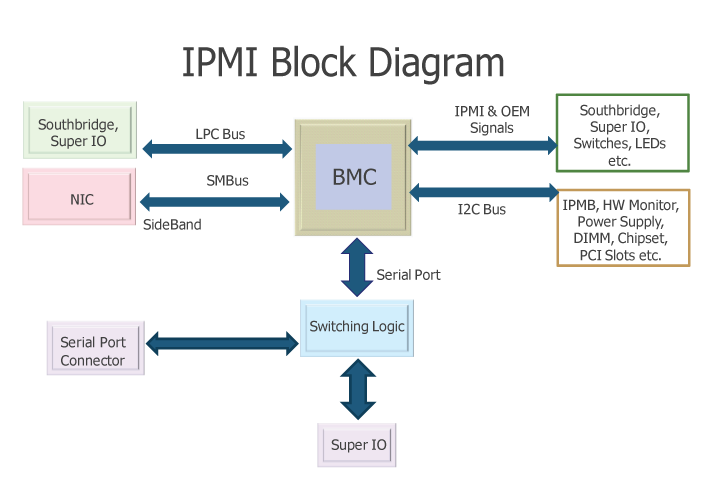
\includegraphics[width=\columnwidth]{figures/IPMI-Block-Diagram.png}}
% \caption{IPMI block diagram, this image was taken from http://pt.wikipedia.org }
% \label{fig:ipmi_diagram}
% \end{figure}

% %The BMC operate independent of the operating system and his access can be through HTTP protocol or using a tool provided by the manufacturer.

The power was collected for all combinations of frequency --- starting from 1.2~GHz and increasing by 100 MHz each time until 2.2~GHz is reached, and possible numbers of active cores --- from 1 to 32. Between each test, the CPU was left idle until it cooled down to avoid interference on the next test.

The coefficients of (\ref{eq_power_final}), $c_1$, $c_2$, $c_3$ and $c_4$, were found by performing multi-linear regression on the data collected. The retrieved fitting can be seen on Fig.~\ref{fig:fitting}.

\begin{figure}[H]
\centerline{\includegraphics[width=\columnwidth]{ch1/figures/power.png}}
\caption{Power model fitting. The dots represent real power measurements and the solid lines represents the modeled power.}
\label{fig:fitting}
\end{figure}

The fitted equation for estimating the power in the target architecture was:
\begin{equation} 
P_{total}(f,p,s)=p(0.29f^3+0.97f)+198.59+9.18s, \label{eq:fittedpower}
\end{equation}
where the unit for frequency is GHz.

To validate this model was calculated the absolute percentage error, i.e. the mean of the perceptual error on each point. This metric was chosen because of the significant difference between the smallest and the biggest values and it is calculated as follows:

\begin{equation}
\sum_{i}^{\rm \# samples}{\frac{|y_i-y_{\rm model}|}{y_i}}.
\label{mpe}
\end{equation}

The resulting minimum, mean, and maximum absolute percentage errors were 0.007\%, 0.75\%, and 2.6\% respectively. While the root mean squared error was 2.38 W.

\subsection{Performance Characterization} \label{sec:performancecharacterization}

To characterize an application, we ran it for all different numbers of active cores in the range of $1<=p<=32$, for all the frequencies in the range of $1.2<=f<=2.2$ using 100MHz steps, and for 5 different input sizes.

%depending on the application, the number of cores was different because some applications can only run with the power of 2 and others can only run with an even number of threads. 
% done, please check \todo[inline]{is this empirically chosen then? What is the reasoning of making such choices?not clear why this selection is useful}
The input sizes were chosen in such a way that the average execution time was in the order of minutes. The sampled power information, on every second, was used to calculate the real energy usage. The total time to complete the characterization varied between one and two days, depending on the application.

The SVR model was built using the collected data. A grid search was used to tune the model parameters. In this case, a Radial Base Function (RBF) kernel and the penalty for the wrong term of $10\times10^3$ and gamma 0.5 \cite{scikit-learn}. To train the SVR, the data collected was divided into two parts, 90\% for training and 10\% to test the accuracy.

The model was validated also using cross-validation $k$-fold with $k$ equal to 10, using the Mean Absolute Error (MAE) and Percentage Absolute Error (PAE) as metrics. The average results of the cross-validation can be seen in Table~\ref{tab:svr_evaluation}.

\begin{table}[H]
\centering
\caption{Performance-Model's Cross validation Errors}
\label{tab:svr_evaluation}
\begin{tabular}{|l|l|l|l|l|}
\hline
Application  & MAE & PAE \\ \hline
\hline
Blackscholes & 2.01  & 4.6\% \\ \hline
Fluidanimate & 6.65  & 1.89\% \\ \hline
Raytrace  & 3.77  & 0.87\% \\ \hline
Swaptions & 2.29  & 2.56\% \\ \hline
\end{tabular}
\end{table}

One of the results of the characterization can be seen in Figs.~\ref{fig:svr_time2}.
% ,~\ref{fig:svr_time3},~\ref{fig:svr_time4}, and ~\ref{fig:svr_time1}.

\begin{figure}[H]
	\centerline{\includegraphics[width=\columnwidth]{ch1/figures/time_fluid_4.png}}
    \caption{Fluidanimate's performance model. The dots represent real performance measurements and the solid lines represent the modeled performance for various numbers of active cores and frequencies when running for input size 3.}
	\label{fig:svr_time2}
\end{figure}

%\begin{figure}[H]
%\subfigure[Fluidanimate's performance model. The dots represent real performance measurements and the solid lines represent the modeled performance.]{%
%	\label{fig:svr_time2}
%	\centerline{\includegraphics[width=\columnwidth]{ch1/figures/time_fluid_4.png}}
%}%
%\end{figure}

% \begin{figure}[H]
% 	\centerline{\includegraphics[width=\columnwidth]{ch1/figures/time_rtview_3.png}}
% 	\caption{Raytrace's performance model. The dots represent real performance measurements and the solid lines represent the modeled performance for various numbers of active cores and frequencies when running for input size 3.}
% 	\label{fig:svr_time3}
% \end{figure}


%\begin{figure}[H]
%\subfigure[Raytrace's performance model. The dots represent real performance measurements and the solid lines represent the modeled performance.]{%
%	\label{fig:svr_time3}
%	\centerline{\includegraphics[width=\columnwidth]{ch1/figures/time_rtview_3.png}}
%}%
%\end{figure}

% \begin{figure}[H]
% 	\centerline{\includegraphics[width=\columnwidth]{ch1/figures/time_swap_3.png}}
% 	\caption{Swaptions's performance model. The dots represent real performance measurements and the solid lines represent the modeled performance for various numbers of active cores and frequencies when running for input size 3.}
% 	\label{fig:svr_time4}
% \end{figure}

%\begin{figure}[H]
%\subfigure[Swaptions performance model. The dots represent real performance measurements and the solid lines represent the modeled performance.]{%
%	\label{fig:svr_time4}
%	\centerline{\includegraphics[width=\columnwidth]{ch1/figures/time_swap_3.png}}
%}%
%\end{figure}

% \begin{figure}[H]
% 	\centerline{\includegraphics[width=\columnwidth]{ch1/figures/time_black_4.png}}
%     \caption{Blackscholes's performance model. The dots represent real performance measurements and the solid lines represent the modeled performance for various numbers of active cores and frequencies when running for input size 3.}
% 	\label{fig:svr_time1}
% \end{figure}

%\begin{figure}[H]
%\subfigure[Blackscholes performance model. The dots represent real performance measurements and the solid lines represent the modeled performance.]{%
%	\label{fig:svr_time1}
%	\centerline{\includegraphics[width=\columnwidth]{ch1/figures/time_black_4.png}}
%}%
%\caption{SVR performance modeling plots for four PARSEC applications. The plots present the modeled and the measured performances for various numbers of active cores and frequencies when running for the mid-size input.}
%\end{figure}
%\todo{mid-size input?}

\section{Experimental Results} \label{sec:experimentsresults}
%As mentioned previously, the aim of this work is to obtain the optimal energy configuration on a parallel application running on a homogeneous platform. In general, the actual solutions are using the DVFS techniques to minimize energy consumption. The following shows the results obtained with the proposed approach.
In this Section, we present results for the energy model that we introduced in Section~\ref{sec:models} based on the parameter fitting described in Sections~\ref{sec:powerfitting} and~\ref{sec:performancecharacterization}. First, we compare and comment on the model in contrast with the actual energy measurements. Finally, we evaluate the effectiveness of the proposed approach by comparing it to the Linux default Ondemand DVFS governor.

\subsection{Measured versus Modeled Energy} \label{sec:measuredversusmodeledenergy}
The energy measurements were obtained by integrating the power measurements over the total execution time of the application.
The power measurements were made using the IPMI sensors with a sampling rate of about one sample per second.
% \todo[inline]{move mode details about IPMI here}

%From energy equation (\ref{eq_energy}), running the parsec applications and using the proposed model, it can be observed a compensation of energy consumption, depending on how application scales, between the growth of the number of cores and the associated decrease on execution time due to the parallelization. So, the results shows that the power consumption does not vary very much, as can see on figures 
Figs. \ref{fig:rt_s3}, and~\ref{fig:swap_s3}
%\ref{fig:fluid_s3}, \ref{fig:black_s3}
plot the measured and modeled energy consumption for Raytrace and Swaptions, respectfully, for varying the number of active cores and operating frequency, running with the mid-size input.

% \begin{figure}[H]
% 	\centerline{\includegraphics[width=\columnwidth]{ch1/figures/fluid_4.png}}
%     \caption{Fluidanimate's energy measurements versus modeled energy consumption  varying the number of active cores and operating frequency, running with the input size 3.}
% 	\label{fig:fluid_s3}
% \end{figure}

%\begin{figure}[H]
%\subfigure[Fluidanimate's energy measurements versus modeled energy consumption]{%
%	\label{fig:fluid_s3}
%	\centerline{\includegraphics[width=\columnwidth]{ch1/figures/fluid_4.png}}
%}%
%\end{figure}


\begin{figure}[h]
	\centerline{\includegraphics[width=\columnwidth]{ch1/figures/rtview_3.png}}
    \caption{Raytrace's energy measurements versus modeled energy consumption  varying the number of active cores and operating frequency, running with the input size 3.}
	\label{fig:rt_s3}
\end{figure}

%\begin{figure}[H]
%\subfigure[Raytrace's energy measurements versus modeled energy consumption]{%
%	\label{fig:rt_s3}
%	\centerline{\includegraphics[width=\columnwidth]{ch1/figures/rtview_3.png}}
%}%
%\end{figure}

\begin{figure}[h]
	\centerline{\includegraphics[width=\columnwidth]{ch1/figures/swap_3.png}}
    \caption{Swaptions's energy measurements versus modeled energy consumption  varying the number of active cores and operating frequency, running with the input size 3.}
	\label{fig:swap_s3}
\end{figure}

%\begin{figure}[H]
%\subfigure[Swaptions' energy measurements versus modeled energy consumption]{%
%	\label{fig:swap_s3}
%	\centerline{\includegraphics[width=\columnwidth]{ch1/figures/swap_3.png}}
%}%
%\end{figure}


% \begin{figure}[H]
% 	\centerline{\includegraphics[width=\columnwidth]{ch1/figures/black_4.png}}
%     \caption{Blackscholes's energy measurements versus modeled energy consumption varying the number of active cores and operating frequency, running with the input size 3.}
% 	\label{fig:black_s3}
% \end{figure}

%\begin{figure}[H]
%\subfigure[Blackscholes' energy measurements versus modeled energy consumption]{%
%	\label{fig:black_s3}
%	\centerline{\includegraphics[width=\columnwidth]{ch1/figures/black_4.png}}
%}%
%\caption{Measured and modeled energy consumption for four PARSEC applications for varying the number of active cores and operating frequency, running with the mid-size input.}
%\end{figure}

%Looking at the same frequency, the energy consumption has greater significance when the program runs with less active cores, but, even the difference being not very significant, the total energy of the best configuration always tend to happen on higher frequency because execution time decreases faster than power increases when raising the frequency. This relation can change depending on the power consumption of the system.
In general, for the case-study applications and case-study architecture, the optimal-energy configurations tend to be the ones using the highest frequency, which characterizes a race-to-idle rather than a pace-to-idle optimal behavior~\cite{kim2015racing}. This can be explained by the large static power observed in the considered architecture, evidenced by the large $c_3$ parameter in (\ref{eq_power_final}) that was fitted in (\ref{eq:fittedpower}). With a large static power, using a pace-to-idle strategy, i.e. the use of frequencies lower than the maximum, is expected to be effective only if the sum of the leakage and the dynamic power parcels is larger than the static power parcel. 
Based on the fitted power model, this would never happen, i.e. the sum of leakage and dynamic power is always less than the static power,
\begin{equation*}
p(0.29f^3+0.97f)+9.18s < 198.59,
\label{ineq:race_to_idle}
\end{equation*}
even if we use the maximum number of cores, $p=32$ and $s=2$, and the maximum frequency, $f=2.2$.

Nevertheless, race-to-idle is not always the best strategy for all systems because energy scales with the execution time, which in turn scales inversely with the number of active cores and the operating frequency, and because power scales linearly with the number of cores, but cubic with the frequency. For this reason, our proposal found optimal strategy for Raytrace and Blackscholes that are not the race-to-idle configuration, as we present in the next Subsection. 

The optimal number of active cores also depends on the parallel scalability of the application. The more scalable the application, the more cores it requires to minimize energy. A scalable application can increasingly exchange the speedup of more cores with lower frequencies in order to spend less energy. This is because of the linear relationship between power and number of cores and the exponential relationship between power and frequency.  

\subsection{Proposed Approach versus Ondemand Linux Governor}
\label{sec:proposedapproach}
We have compared the energy consumption of the four case-study applications using the energy-optimal configurations provided by the proposed approach to the energy consumption resulted by use of the Linux default DVFS governor, Ondemand. Since the governor does not choose the number of active cores, we executed each application using 1, 2, 4, 6, 8, $\cdots$, 28, 30, and 32 cores, accounting for the best and the worst cases of energy consumption. Tables \ref{tab:fluidfreq}, \ref{tab:raytracefreq}, \ref{tab:swapfreq} and \ref{tab:blackfreq} present these results for Fuidanimate, Raytrace, Swaptions, and Blackscholes, respectively. the maximum and minimum savings of the proposed approach in comparison with the Ondemand governor. The savings are calculated as follows: 
\begin{equation}
    \frac{100*({\rm Proposed}-{\rm Ondemand})}{\rm Ondemand}.
\end{equation}

\begin{table}[H]
\caption{Fluidanimate Minimal energy}
\label{tab:fluidfreq}
\resizebox{\columnwidth}{!}{%
\begin{tabular}{l|l|l|l|l|l|l|ll}
Input & \rot{\begin{tabular}[c]{@{}l@{}}Mean Freq. \\ in GHz \\ (\#Cores) \end{tabular}} & \rot{Energy in KJ} & \rot{\begin{tabular}[c]{@{}l@{}}Mean Freq. \\ in GHz \\ (\#Cores) \end{tabular}} & \rot{Energy in KJ} & \rot{\begin{tabular}[c]{@{}l@{}} Freq. \\ in GHz \\ (\#Cores) \end{tabular}} & \rot{Energy in KJ} & \multicolumn{1}{l|}{\rot{Min. Save(\%)}} & \rot{Max. Save(\%)} \\ \hline
1     & 1.85 (32)                                                                        & 4.85               & 2.29 (1)                                                                         & 32.38              & 2.0 (32)                                                                     & 4.15               & \multicolumn{1}{l|}{14.5}                & 87.2                \\ \hline
2     & 1.88  (32)                                                                       & 9.35               & 2.29 (1)                                                                         & 66.77              & 2.0 (32)                                                                     & 7.89               & \multicolumn{1}{l|}{15.7}                & 88.2                \\ \hline
3     & 1.89  (32)                                                                       & 18.82              & 2.30 (1)                                                                         & 135.00             & 2.0 (32)                                                                     & 16.98              & \multicolumn{1}{l|}{9.8}                 & 87.4                \\ \hline
4     & 2.08  (32)                                                                       & 37.80              & 2.30 (1)                                                                         & 272.55             & 2.1 (32)                                                                     & 33.20              & \multicolumn{1}{l|}{12.2}                & 87.8                \\ \hline
5     & 2.00  (32)                                                                       & 76.28              & 2.30 (1)                                                                         & 546.84             & 2.2 (32)                                                                     & 66.83              & \multicolumn{1}{l|}{12.4}                & 87.8                \\ \hline
      & \multicolumn{2}{l|}{Ondemand Min.}                                                                    & \multicolumn{2}{l|}{Ondemand Max.}                                                                    & \multicolumn{2}{l|}{Proposed}                                                                     &                                          &                    
\end{tabular}
}
\end{table}

\begin{table}[H]
\caption{Raytrace Minimal energy}
\label{tab:raytracefreq}
\resizebox{\columnwidth}{!}{%
\begin{tabular}{l|l|l|l|l|l|l|ll}
Input & \rot{\begin{tabular}[c]{@{}l@{}}Mean Freq. \\ in GHz \\ (\#Cores) \end{tabular}} & \rot{Energy in KJ} & \rot{\begin{tabular}[c]{@{}l@{}}Mean Freq. \\ in GHz \\ (\#Cores) \end{tabular}} & \rot{Energy in KJ} & \rot{\begin{tabular}[c]{@{}l@{}} Freq. \\ in GHz \\ (\#Cores) \end{tabular}} & \rot{Energy in KJ} & \multicolumn{1}{l|}{\rot{Save Min.(\%)}} & \rot{Save Max.(\%)} \\ \hline
1     & 1.30 (4)                                                                         & 38.56              & 2.29 (1)                                                                         & 60.29              & 2.2 (6)                                                                      & 37.92              & \multicolumn{1}{l|}{1.7}                 & 37.1                \\ \hline
2     & 1.32 (8)                                                                         & 43.59              & 2.30 (1)                                                                         & 98.11              & 2.2 (10)                                                                     & 39.93              & \multicolumn{1}{l|}{8.4}                 & 59.3                \\ \hline
3     & 1.65 (16)                                                                        & 49.40              & 2.30 (1)                                                                         & 168.82             & 2.2 (14)                                                                     & 45.77              & \multicolumn{1}{l|}{7.4}                 & 72.9                \\ \hline
4     & 1.62 (32)                                                                        & 55.61              & 2.30 (1)                                                                         & 299.83             & 2.2 (22)                                                                     & 52.99              & \multicolumn{1}{l|}{4.7}                 & 82.3                \\ \hline
5     & 1.77 (32)                                                                        & 69.33              & 2.30 (1)                                                                         & 520.34             & 2.2 (26)                                                                     & 67.28              & \multicolumn{1}{l|}{3.0}                 & 87.1                \\ \hline
      & \multicolumn{2}{l|}{Ondemand Min.}                                                                    & \multicolumn{2}{l|}{Ondemand Max.}                                                                    & \multicolumn{2}{l|}{Proposed}                                                                     &                                          &                    
\end{tabular}
}
\end{table}

\begin{table}[H]
\caption{Swaptions Minimal energy}
\label{tab:swapfreq}
\resizebox{\columnwidth}{!}{%
\begin{tabular}{l|l|l|l|l|l|l|ll}
Input & \rot{\begin{tabular}[c]{@{}l@{}}Mean Freq. \\ in GHz \\ (\#Cores) \end{tabular}} & \rot{Energy in KJ} & \rot{\begin{tabular}[c]{@{}l@{}}Mean Freq. \\ in GHz \\ (\#Cores) \end{tabular}} & \rot{Energy in KJ} & \rot{\begin{tabular}[c]{@{}l@{}} Freq. \\ in GHz \\ (\#Cores) \end{tabular}} & \rot{Energy in KJ} & \multicolumn{1}{l|}{\rot{Min. Save(\%)}} & \rot{Max. Save(\%)} \\ \hline
1     & 2.15 (32)                                                                        & 5.88               & 2.29 (1)                                                                         & 80.08              & 2.2 (32)                                                                     & 5.73               & \multicolumn{1}{l|}{2.5}                 & 92.8                \\ \hline
2     & 2.00 (32)                                                                        & 9,21               & 2.30 (1)                                                                         & 106.84             & 2.2 (32)                                                                     & 7,81               & \multicolumn{1}{l|}{15.2}                & 92.7                \\ \hline
3     & 2.22 (32)                                                                        & 10.37              & 2.30 (1)                                                                         & 133.41             & 2.0 (32)                                                                     & 9.90               & \multicolumn{1}{l|}{4.5}                 & 92.6                \\ \hline
4     & 2.02 (32)                                                                        & 14.29              & 2.30 (1)                                                                         & 160.34             & 2.0 (32)                                                                     & 12.33              & \multicolumn{1}{l|}{13.8}                & 92.3                \\ \hline
5     & 2.08 (32)                                                                        & 15.82              & 2.30 (1)                                                                         & 186.39             & 1.9 (32)                                                                     & 14.45              & \multicolumn{1}{l|}{8.7}                 & 92.2                \\ \hline
      & \multicolumn{2}{l|}{Ondemand Min.}                                                                    & \multicolumn{2}{l|}{Ondemand Max.}                                                                    & \multicolumn{2}{l|}{Proposed}                                                                     &                                          &                    
\end{tabular}
}
\end{table}
\begin{table}[H]
\caption{Balckschoels Minimal energy}
\label{tab:blackfreq}
\resizebox{\columnwidth}{!}{%
\begin{tabular}{l|l|l|l|l|l|l|ll}
Input & \rot{\begin{tabular}[c]{@{}l@{}}Mean Freq. \\ in GHz \\ (\#Cores) \end{tabular}} & \rot{Energy in KJ} & \rot{\begin{tabular}[c]{@{}l@{}}Mean Freq. \\ in GHz \\ (\#Cores) \end{tabular}} & \rot{Energy in KJ} & \rot{\begin{tabular}[c]{@{}l@{}} Freq. \\ in GHz \\ (\#Cores) \end{tabular}} & \rot{Energy in KJ} & \multicolumn{1}{l|}{\rot{Min. Save (\%)}} & \rot{Max. Save(\%)} \\ \hline
1     & 1.57 (32)                                                                        & 1.36               & 2.27 (1)                                                                         & 16.35              & 2.2 (30)                                                                     & 1.69               & \multicolumn{1}{l|}{-23.9}                & 89.7                \\ \hline
2     & 2.09 (32)                                                                        & 2.93               & 2.24  (1)                                                                        & 33.16              & 1.8 (32)                                                                     & 3.36               & \multicolumn{1}{l|}{-14.7}                & 89.9                \\ \hline
3     & 1.82 (32)                                                                        & 8.08               & 2.23  (1)                                                                        & 65.97              & 2.2 (30)                                                                     & 6.55               & \multicolumn{1}{l|}{18.9}                 & 90.1                \\ \hline
4     & 2.01 (32)                                                                        & 12.59              & 2.14  (1)                                                                        & 131.85             & 2.2 (26)                                                                     & 13.64              & \multicolumn{1}{l|}{-8.3}                 & 89.7                \\ \hline
5     & 1.97 (32)                                                                        & 25.29              & 1.57  (1)                                                                        & 263.89             & 2.2 (28)                                                                     & 26.52              & \multicolumn{1}{l|}{-4.8}                 & 90.0                \\ \hline
      & \multicolumn{2}{l|}{Ondemand Min.}                                                                    & \multicolumn{2}{l|}{Ondemand Max.}                                                                    & \multicolumn{2}{l|}{Proposed}                                                                     &                                           &                    
\end{tabular}
}
\end{table}

In most cases, the proposed approach obtained better results than the best cases of the Ondemand governor. For Blackscholes, the proposed approach was only better than the Ondemand best case for input number 3. On average, the proposed method was 5.7\% better than the best case of the Ondemand governor.
%This can be explained by the linear speedup characteristic of this application. Thus, it is to be expected that on constant efficiency, the better solution will be with more cores.

%The other results on the other applications show that the proposed approach, even in cases on the bests configurations for DVFS, demonstrate that can obtain energy saving of up 18\%, comparing to the Ondemand governor. 
In all cases, the method proposed here outperformed the worst case of the Ondemand governor. On average, the difference in energy consumption was about 88.8\%, being 92.8\% the maximum difference and 37.1\% the minimum. In general, the energy consumption of the DFVS scheme was larger for smaller numbers of cores. Nonetheless, it was not always the case that the best number of cores for this scheme was the maximum, i.e. 32 cores. Possibly, for architectures with larger number of cores, choosing the exact number the minimizes energy consumption would be less evident.


Fig. \ref{fig:energy_results} shows the behavior of the energy consumption for some tested cases of the Ondemand governor. The presented values are normalized to the energy consumption of the proposed approach.

\begin{figure}[H]
    \centering
    \subfloat[Fluidanimate]{
        \includegraphics[width=\columnwidth]{ch1/figures/fluid.png}
        \label{fig:com_fluid}
    }
	\\
    \subfloat[Raytrace]{
        \includegraphics[width=\columnwidth]{ch1/figures/rtview.png}
        \label{fig:com_rtview}
    }
	\\
    \subfloat[Swaptions]{
        \includegraphics[width=\columnwidth]{ch1/figures/swap.png}
        \label{fig:com_swap}
    }
	\\
    \subfloat[BlackScholes]{
        \includegraphics[width=\columnwidth]{ch1/figures/black.png}
        \label{fig:com_black}
    }
    \caption{Energy consumption of the Ondemand governor for power-of-2 numbers of cores and the proposed approach. The values are relative to the energy of the proposed approach.}
    \label{fig:energy_results}
\end{figure}


%%%% moved to the conclusions.
% A weak of this approach is that the model of performance and power needed to be trained with previously known input sizes. This weakness can be treated with a future solution that can incorporate a prediction of input size during execution of the application. 

% Although, the results demonstrate to be very interesting because it is achieved better results for all inputs sizes on 3 out of 4 applications as can see on \ref{fig:com_fluid}, \ref{fig:com_rtview} and \ref{fig:com_swap}. Also for Fluidanimate and Raytrace the mean energy saving compared to the best result of Ondemand was higher then 10\%. On the overall mean, we save 6\% of energy.

\section{Related Work} \label{sec:relatedwork}
DVFS is the most common technique employed to obtain energy savings on multi-core systems. Thus, the technique has been extensively researched with the aim of providing strategies for selecting the optimal voltage and frequency for a specific application and architecture. In \cite{Anghel2011} the authors utilized two algorithms for scaling the frequency of the processors: a human-immune system inspired algorithm to monitor the server's power and performance states; and fuzzy logic based algorithm for changing the server's performance state. \cite{Cochran2011} introduced a scaling method for determining the system's optimal operation points for the number of threads and DVFS settings.

In \cite{DaCosta2015}, an approach that considers instantaneous system activity states was proposed. In this case, the memory and network activity were used to generate a DVFS management setting.

Performance counters have also been used to perform effective DVFS. In \cite{Spiliopoulos2011}, the authors used a Continuous Adaptive DVFS based on a performance model of the processor. The model was based on sampling the hardware's performance counters at regular intervals to predict performance/energy workloads. Base on these predictions appropriate voltage, and frequency settings were selected.

In this work, we introduce a power and a performance model to find energy-optimal operating frequency and number of active cores for applications running on specific multi-core platforms. Our approach does not use the DVFS manager to control the processor voltage and frequency settings. This new approach can obtain better results than DVFS strategies as was shown in \cref{sec:experimentsresults}. 

The success obtained from this approach is possible due to the fact that the use previous knowledge of the application's performance on the target architecture can expose sufficiently relevant information, such as parallel speedups, that is harder to guess in runtime techniques based on DVFS.

The use of an application-agnostic power modeling for the target architecture helps to make the technique portable to other applications. That is, to estimate the energy-optimal frequency and number of active cores for a new application, only a performance characterization is needed.
%\todo[inline]{I have edited the related work section. The last two sentence starting from "Our approach..." need to be edited. You need to put why our technique is different and why is better. Saying that our results are better is not wise, with out providing the savings achieved by the other techniques.}

\section{Conclusion and future work} \label{sec:conclusion}
In this paper, we propose a new approach to optimize the energy efficiency of single-node batch HPC applications. In contrast to existing scheduling algorithms, our technique utilizes the application's runtime profile, and a power model of the compute node to predict the optimal frequency and number of cores to be used. This proven effective in reducing the energy consumption of applications. 

In contrast to conventional DVFS schemes, out approach chooses not only the operating frequency, but also the number of cores to run an application. DVFS schemes leave to the user the choice of how many cores to use, which becomes harder take with the increase in processor core counts.

Results from four parallel PARSEC applications running on an HPC node with two sixteen-core processors show that the novel approach outperforms the default Linux DVFS scheme on its best case with an average of 5.7\% energy savings. In its worst case, the savings were about 88.8\%, on average. The former represents the case when the user would have an oracle to disclosure the optimal number of cores to run the application. The latter often falls into the single-core usage, which is a common choice of many regular users of batch single-node jobs in HPC.


% In high-performance computing systems shared by multiple users normally on Universities and research centers. The user demands his necessary resources needed for the job. With our approach, the users can choose to finish the job while saving energy and the scheduler will choose the necessary resources. For example, if we assume that the choice of the number of cores varies with a random uniform distribution when compared with our method we could save about 18\%. Another common usage of the system is to use only one core which tends to be the worst case as shown in \ref{fig:energy_results}, in this case, we could save around 88.8\%, depending on the user's profile.

A weakness of the proposed technique is the need for information about the input size of the application before execution. A possible solution would be to use performance counters, present in all modern HPC processors, to guess the input size based on previously trained data.

Future work will improve the proposed energy model by taking into account more relevant information, such as the percentage of CPU utilization. This can enable the identification of different phases of the target program and thus, it will enable more fine-grained changes of the frequency and, perhaps, the number of active cores, to further improve the results presented here.
%Furthermore, since the Ondemand governor is not able to select the number of cores, this choice is left to the user, if the application allows. In contrast, the proposed approach automatically uses the number of cores and frequency to reduce energy consumption.


% \newpage
% \appendix

% This appendix shows the steps necessaries to aim reproduce the experiments of this work.

% \section*{Artefact Description}
% Our artifact provides scripts that can reproduce the experiments in this paper. You can download them at a public repository on GitHub. There is a Python Virtual environment and 4 scripts to use.

% The requirements necessary to reproduce this results is a system with a Linux kernel, super user access configured, the acpi-cpufreq driver and the IPMI system and the PARSEC 3.0 Benchmark installed on system. To setup this environment, you can run:

% \begin{lstlisting}[language=bash,caption={Setup}]
% git clone https://github.com/Teste899/SC18
% cd SC18/
% source sc18/bin/activate$
% \end{lstlisting}

% The scripts available are:
% \begin{enumerate}
% \item{$power\_monitor:$ collect power information using IPMI and a program to stress the CPU to the maximum.}
% \item{$power\_fitting:$ calculates the power model constants of the system and compute the errors using data from the $power\_monitor$.}
% \item{$performance\_monitor:$ makes the complete modeling from the collection of execution times to the calculation of the SVR.}
% \item{$performance\_fitting:$ use the SVR model and the power model to compute the energy and find the minimal energy configuration.}
% \end{enumerate}

% Each script has its own parameters that are detailed using -h option 

% \begin{lstlisting}[language=bash,caption={Scripts}]
% python power_monitor.py -h
% python power_fitting.py -h
% python performance_monitor.py -h
% python performance_fitting.py -h
% \end{lstlisting}

% The input arguments used on the applications was:

% \begin{lstlisting}[language=bash,caption={Applications input arguments}]
% Blackscholes
% '_nt_', 'in_625K.txt', 'out_625K.txt'
% '_nt_', 'in_1M.txt', 'out_1M.txt'
% '_nt_', 'in_2M.txt', 'out_2M.txt' 
% '_nt_', 'in_5M.txt', 'out_5M.txt'
% '_nt_', 'in_10M.txt', 'out_10M.txt'


% Fluidanimate
% '_nt_', '250', 'in_500K.fluid'
% '_nt_', '500', 'in_500K.fluid'
% '_nt_', '1000', 'in_500K.fluid'
% '_nt_', '2000', 'in_500K.fluid'
% '_nt_', '4000', 'in_500K.fluid'

% Raytrace
% 'thai_statue.obj','-automove', '-nthreads',
% '_nt_', '-frames', '10000', '-res', '140', '140'
% 'thai_statue.obj','-automove', '-nthreads',
% '_nt_', '-frames', '10000', '-res', '196', '196'
% 'thai_statue.obj','-automove', '-nthreads',
% '_nt_', '-frames', '10000', '-res', '274', '274'
% 'thai_statue.obj','-automove', '-nthreads',
% '_nt_', '-frames', '10000', '-res', '384', '384'
% 'thai_statue.obj','-automove', '-nthreads',
% '_nt_', '-frames', '10000', '-res', '537', '537'

% Swaptions
% '-ns', '64', '-sm', '3000000', '-nt', '_nt_'
% '-ns', '64', '-sm', '4000000', '-nt', '_nt_'
% '-ns', '64', '-sm', '5000000', '-nt', '_nt_'
% '-ns', '64', '-sm', '6000000', '-nt', '_nt_'
% '-ns', '64', '-sm', '7000000', '-nt', '_nt_'
% \end{lstlisting}

% The PARSEC 3.0 Benchmark and its necessary input files are available at http://parsec.cs.princeton.edu/download.htm.

% \section*{Execution order}
% The monitoring scripts must first be run to collect the necessary data for be used by fitting scripts. A execution example of the power script is:

% \begin{lstlisting}[language=bash,caption={Power scripts}]
% python power_monitor.py 1,2,4,8,10,12 \ 
%                         16 60 30 power_model
% python power_fitting.py power_model
% \end{lstlisting}

% This script will collect power information and to perform the model fitting and its validation. 

% \begin{lstlisting}[language=bash,caption={Performance scripts}]
% python2.7 performance_monitor.py cpu_load 
% "16,32" 32 "nt_ 5,_nt_ 10" 1 10
% python2.7 performance_fitting.py cpu_load 1
% \end{lstlisting}

% The performance scripts will also collect data of the power consumption and execution time. From the execution time it is going to calculate the SVR estimation and perform a cross validation. The energy equation its also calculated there using the power model previously calculated and all the results can be dynamically observed.

